\documentclass[twocolumn]{article}
\usepackage[pdftex]{graphicx}
\usepackage{amsmath}
\usepackage{parskip}
\author{Michael Anderson, Dale Cox, Karl Smeltzer, Zachary Sommers,
Justin Wolford}
\title{A Brief Survey of Results from the DNA Computing Field}
\begin{document}
\maketitle
\hyphenpenalty=10000

\vspace{3em}

\begin{abstract}
In this paper we give an overview of the biological foundations, problems, and
possible applications associated with the emerging field of DNA computing. We
begin by pointing out that the end is in sight for Moore's Law unless classical
computers are supplemented or replaced by other types of computing technology.
We then summarize the biochemical oddities of DNA that allow for
computation using it to be a possibility, and a couple of known methods for
using it to simulate Turing Machines. We discuss some problems with this
technology that have been found by attempting to put it into practice, such as 
the chemical errors that are responsible for the mutation and evolution of
life. Finally, we conclude that baring any monumental field-changing insights,
DNA will not replace classical computers for general purpose computation, but
it may prove useful for specific applications in biomedicine or nano-technology.
\end{abstract}

\section{Introduction}
For the last several decades the speed and compactness of computing technology
has increased exponentially in rough accord with Moore's Law. However,
exponential growth cannot continue indefinitely, and in particular the speed of a
classical computer with integrated circuitry is bounded by certain physical
constants. For example, since the propagation time of electrical signals is
fixed at the speed of light, decreasing the cycle time of a processor requires
transistors to become smaller and more tightly crammed together. The problem of
course is that we cannot imagine transistors that are smaller than a molecule,
and molecules are only so small. The width of an atom, which would be the
absolute lowest bound on the size of a transistor, is on the order of 0.1 nm,
and in the last decade we have developed CPUs with transistors on the order of
only 10nm \cite{rama}.

Since huge improvements in the performance of classical computing systems
seems to be close to an end,
many researchers are looking into a variety of radically different physical
models for computation, such as quantum computing and optical computing. The
possibility we investigate here is the still emerging field of DNA computing.

\section{Biological Background}
The current model of DNA computing was first put forth by Leonard
Adleman in an article he published in ``Science'' in 1994. While
researchers such as Charles Bennett and Rolf Landauer had been
considering the physical limitations of transistor-based computers and
possible alternatives (including DNA) much earlier \cite{bennett},
Adleman was the
first to bring more recent biological discoveries together into a
working model \cite{adleman_98}.

Adleman's model was fundamentally based on the properties of DNA
polymerase, an enzyme critical in the process of DNA replication. When
put in contact with a strand of DNA in solution, DNA polymerase will
produce a second strand with a different structure in which each of
the bases is replaced by its Watson-Crick complement \cite{watson}. When two
complementary strands come into contact, they anneal, forming hydrogen
bonds at each of the matching pairs \cite{winfree_95}. Adleman compared this
process
to the function of a Turing machine, reading bases from a tape and
writing their respective complements into the output \cite{adleman_98}.

Adleman also saw a computational use for DNA nucleases and ligases,
enzymes which cut a strand at a predetermined sequence and covalently
bond two strands into a single, longer strand respectively \cite{adleman_94}.

DNA molecules in a gel solution can be forced to undergo a type of
sorting operation, in which longer strands are separated from shorter
ones. This is done through gel electrophoresis, a technique in which
current is applied to the solution and the negatively charged DNA
molecules move toward the electrode. Shorter strands move more quickly
than longer strands, and thus sort themselves by size \cite{lodesh}.

Adleman then demonstrated the ability to solve combinatorial problems
with these principles and techniques, using the Hamiltonian path
problem as an example. He first carefully designed the problem,
assigning a DNA sequence comprised of two parts to each node in the
graph, as well as a sequence for each existing edge made up of the
second part of the origin node sequence and the first part of the
destination node sequence concatenated together \cite{adleman_94}.

The next step was simply to synthesize DNA molecules from the edge
sequences and the complements of the node sequences. This allowed the
edge molecules to join with their assigned connected nodes at the
complementary section, and eventually construct longer, more complex
strands through repeated bonding. This generated DNA molecules
representing all the possible paths through the graph \cite{adleman_94}.

Using the two short DNA primer strands representing the start and end
nodes, Adleman was able to create a controlled polymerase chain
reaction which produced copies of strands with correct start and end
points exponentially fast, while ignoring the incorrect strands
\cite{adleman_98}.

Through a series of separation procedures, Adleman was able to extract
only those strands which passed through each node on the graph, and
was able to determine both if a Hamiltonian path existed (if any DNA
molecules are remaining) and which is the shortest through the use of
gel electrophoresis \cite{adleman_94}.

This or a similar process can theoretically
represent any Turing machine, and solve any Turing-computable problem
given enough of the restriction enzymes \cite{wilhelm}.

\section{Example Turing Machine Implementation}
Qian, Soloveichik, and Winfree proposed one way of using DNA to
create a Turing-complete computation system \cite{qian}. Instead of directly
implementing a Turing machine, their proposal involves a multiple
stack system that is Turing complete and as efficient as multi-tape
Turing machines \cite{minsky}. This decision relates to DNA polymers lending
themselves more readily to creating stacks than traditional Turing
tapes.

The basic structure consists of one or more stack polymers where each
molecule represents a particular letter $x \in \Sigma$. Chemical reaction
networks are used as state transitions, adding and removing molecules
from the stack. Importantly, this is done in a way that is reversible,
which allows a particular addition or removal to be undone without
adding to the energy cost \cite{qian}.

Reactions rely on a DNA fuel species that is specific to a particular
DNA molecule. For example, fuel species F$_{1X}$ applies only to attaching
molecule X to the stack 1 polymer. Additionally, each time a molecule
is added to the stack, it releases a confirmations molecule (Q) that
is used later when querying the stack. This Q molecule is also easily
changed from a stack specific molecule (Q$_1$) to a generic form.

The stack consists of a polymer with a fixed end and a growing end.
The fixed end is denoted with a special molecule that indicates an
empty stack. Molecules are added to the stack when both the correct
fuel and molecule are present. It is worth noting that several fuels
may be attempted unsuccessfully before the correct match is made. If a
fuel (specific to a particular stack) attempts to bond with that stack
polymer, it will only succeed if the correct input molecule is present
as well. For instance, any fuel F$_{1Y}$ may attempt to bond with stack 1,
but will fail if molecule X instead of Y is present. This can result
in many fuel attempts before F$_{1X}$ successfully bonds X to the growing
end of stack 1.

For an example computation, consider an input polymer (S$_1$) that is to
be copied to two output polymers (S$_2$ and S$_3$) using an alphabet of
$\{0,1\}$. The state transitions consist generally of popping S$_1$ and
copying that molecule to S$_2$ then S$_3$.  Using the Q molecule, the top
element of S$_1$ is removed. This leads to the states where molecules
representing that same element are added to S$_2$ and S$_3$, creating their
own Q confirmation molecules. This process is repeated until S$_1$
reaches the empty stack molecule. There is an illustration of this process in
Fig. 1.

\vspace{2em}

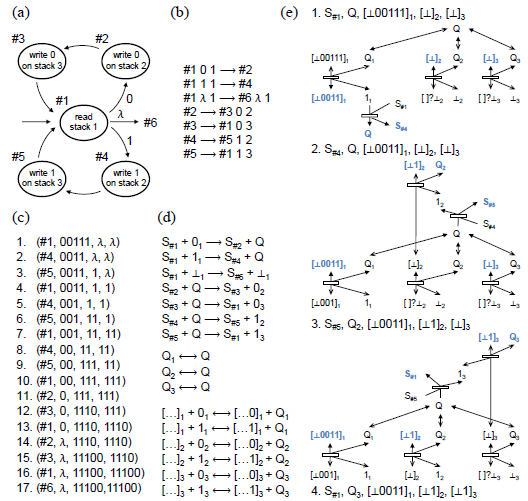
\includegraphics[scale=0.43]{zach2.png}
\begin{center}Fig. 1 \cite{qian}\end{center}

\vspace{2em}

This is only one example from the overall field and there are
drawbacks to this method as well as advantages. The reversible
reactions are more efficient than having two irreversible forward/back
reactions, which is a considerable advantage. However, the need to
have unique free-floating polymers (stacks) in the same solution
limits the scope and parallelization of this method. Additionally,
some other methods are able to use complete material recycling outside
of the computation output, while this approach consumes materials.

\section{Errors and Tile Computing}
In basic DNA computing there are two varieties of errors, Type I and Type II.
 Type I errors are false negative errors. At some stage in the filtration 
process, some matching string was misidentified as not matching and was removed
from the sample. This is the worst kind of error because it is impossible to 
recover that strand again. The other type of error, Type II, occurs when some 
non-matching strand is mistakenly matched. This simply means that we have 
carried over some strand when we should not have. This is not as bad as the 
first because there is a chance the strand will be later filtered out
\cite{boneh}.

Many forms of DNA computing require filtering of DNA strands based on their 
composition. Most operations in DNA computing involve extracting strands that 
match a particular pattern. However, it may be considered acceptable to miss 
5\% of the strands matching a pattern. This means that if a particular “good” 
strand goes through 100 extraction operations there is only 0.5\% chance that 
it will still remain even though it was what was looked for. This is a 
significant problem facing DNA computing. One possible solution is to add 
additional steps to the screening process. Boneh et al. suggest a constant 
volume process where the strands are doubled every time half of the material 
is weeded out. This will help ensure that a good strand survives. However it 
adds significant time to the final detection step because one may need to test 
many strands to see if they are a solution to the problem \cite{boneh}.

Another solution to help with filtering is the double encoding of data. This 
essentially gives the filtering process two places to match to every string, 
increasing the chance that good strings will survive a filtering process. 
However, this also requires that strands be twice as long so there may only be 
half as many strands. Depending on the number of extractions and the increased 
probability of survival by having doubly encoded data, this can help reduce 
false negatives \cite{boneh}.

Another promising approach to DNA computing is tile self assembly. Winfree has 
shown that tile self assembly in DNA computing is Turing universal
\cite{winfree_98}. It may 
also be more practical than other means of DNA computing because the smallest 
blocks are self assembled instead of being manipulated in some fashion. 

Different kinds of errors are associated with DNA self assembly. There are 
growth errors, facet errors and nucleation errors. Growth errors happen when a 
DNA tile “sticks” someplace  where a different tile should be. A facet error 
occurs when a tile attaches where no tile is supposed to attach and a 
nucleation error occurs when two free floating tiles attach separate from the 
seed structure \cite{chen_04} \cite{chen}.

One proposed solution is to make tiles more unique. So where a tile may have 
used only two glues previously, we replace those glues with a more unique
combination.

\vspace{1em}

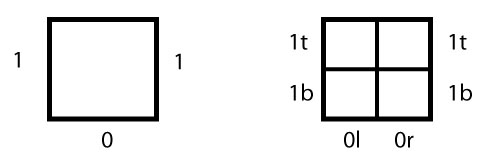
\includegraphics[scale=0.47]{moreGlue.png}
\begin{center}Fig. 2\end{center}

\vspace{1em}

For example, in Fig. 2, we replaced the 1 glue with a 1t and 1b glue and we 
replaced the 0 glue with a 0l and a 0r glue. Now, for a tile to incorrectly 
bind to this tile it will need to bind to two incorrect locations instead of 
just one \cite{chen_04}. The problem is that this has just doubled the
complexity of our 
tiles and has also increased the space required to solve the problem.

Another solution proposed by Chen and Kao is to optimize the concentration of
tiles based on the expected tile assembly. They suggest that the correct ratio
of 
tiles to introduce into the system is the square root of the expected ratio of 
tiles \cite{chen}. So if we are using two tiles X and Y, and we expect to end
with a 
ratio of 25:1 tiles, then the concentration of tiles we use when supplying
tiles
to assemble should be 5:1. They admit that these concentrations may vary 
greatly from the ideal concentration of tiles required to assemble the tiles 
quickly. So we have essentially traded time for errors in this situation. They
also fail to address the problem that one needs to know the final ratio in 
order to determine the correct concentration.


\section{Applicability}
Although the field is still in its infancy, there have already been
impressive breakthroughs demonstrating applications of DNA computers.
Two obvious advantages of DNA computing are its massive parallelism
and extremely dense storage capacity. While the potential is great,
there are major hurdles that need to be overcome if DNA computing will
ever become feasible.

Since Adleman's initial experiment, researchers have found new
methods and uses for DNA computing. Shapiro and Beninson have produced
a DNA automaton which detects cancerous cells and can release a drug
when an infected cell is found \cite{shapiro}. Although this experiment was
only
performed in a test tube, the next goal is living cells. Eric Winfree
has developed a method for building ``molecular tiles'' which could
allow for complex self-assembling molecular structures 
\cite{parker}. This would be a major advancement for areas like nanotechnology.

The sheer computational advantage of DNA computing is easy to see;
Adleman's TSP experiment ran at the equivalent of 100 Teraflops
\cite{parker}.
This processing speed comes from the parallelism inherent in DNA
computing, the speed is proportional to the number of DNA molecules
present.  As a storage medium, DNA is very dense and capable of storing
massive amounts of data. As an example, 1μmol of DNA in 1L of water
contains $10^{18}$ strands of DNA and each strand has a length of 40 which
can encode 10 bytes \cite{kari}. This means 1L of solution has the potential
to store around 8.7 exabytes.

Some problems are still not
easily solvable even with seemingly boundless computing power and
memory. If Adleman's experiment was scaled up to 200 cities, it is
estimated the weight of the DNA required to represent all possible
routes would be more than the earth 
\cite{parker}. Another problem is obtaining
the output of the computations; it took Adleman a week to extract the
solution to his TSP experiment \cite{parker}.

As for the power efficiency of DNA computers, it is leaps ahead of current
technology. IBM's recent Blue Gene supercomputer which is considered
to be highly efficient runs at 1684 megaFLOPS/watt \cite{drew}. It was
estimated by Adleman that a DNA based computer could achieve 20
petaFLOPS/watt \cite{kari}.

\section{Conclusion}

Remarkable as it may seem, it has been shown that the same sort of processes
that operate on the DNA within every living cell can be used to do
Turing-complete computation by at least the two methods mentioned above:
a stack-based method and a tiling-based method. Additionally, in theory DNA
offers massively
parallel computation, very efficient power consumption, and high-density memory
storage.

Unfortunately, DNA computation is non-deterministic in the most undesirable
sense, as the same sort of copying and bonding errors that cause cancer in life
can randomly cause any DNA program to give garbage output. Furthermore, it is
not known if and how
the models of DNA computation that we have right now can scale effectively
enough to solve the sort of complex and practical problems that we can
currently solve using classical computers.

All in all, there are trade-offs for both DNA computers and current
silicon-based
systems. As a general computing platform, the consensus is that DNA
computers will never directly replace silicon-based systems 
\cite{parker}. Amos
suggests we shouldn't be looking at the two as competitors but we
should be ``looking outside the box for a niche for other application''
\cite{parker}. Because DNA computers speak the language of living cells, they
can accomplish tasks that silicon systems will never be able to, particularly
for applications in molecular robotics, cancer diagnosis, and nano-technology.
It is
envisaged that DNA computers will act more as a complement, rather
than a replacement, to classical computing \cite{kari}.

If nothing else, even the fact that the properties of DNA can in theory be
used to make something as powerful as
a classical computer is interesting, and adds to the knowledge-base of
theoretical computer science. Furthermore, we may eventually develop or
discover
other systems in nature that have properties similar to DNA, but happen to be
more amenable to general purpose computation, for which we can put the
theory into practice.

\newpage

\bibliography{dna_computing}{}
\bibliographystyle{plain}
\end{document}
